\chapter{Amélioration du diagnostic image}
\label{chap:chapter_5}
\chapterintro
Lors de la précédente partie nous avons présenté des schéma de classification adapté aux données de \gls{rcm}, au sein de schéma "classique" qui traitent l'information comme donnée unique.\par

Ce second chapitre dédié aux approches \gls{rcm} nous permettra de mettre en avant divers schéma de classification autres.\par

\newpage

\section{Méthodologie}
Lors du précédent chapitre nous avons pu déterminer un certain nombre de pistes permettant de traiter au mieux\par

Afin de tenter de résoudre cette problématique, nous nous intéresserons à une continuité des méthodes précédentes par approche de classification "classique", puis nous aborderons le problème à l'aide d'approche d'apprentissage profond de bout en bout.\par

\section{Approche par apprentissage automatique}
A l'aide cette partie nous étendrons les méthodes précédentes dans le but d'améliorer la précision du diagnostic. Nous nous sommes pour cela inspiré de deux principaux mode d'approches: une approche par multiple résolution que nous détaillerons dans une première sous partie et une approche par prédiction locales que nous énoncerons dans une seconde sous partie.\par

\subsection{Approche par multiples échelles}
L'un des constats concernant les données \gls{rcm} en notre possession est que cette information est relativement régulière. En effet, les spécialistes ont pour l'acquisition de ces données conservée des paramètres similaires, y compris sur la provenance et la taille des acquisitions. Ainsi, les données sont homogènes d'un point de vue spatial.\par

Néanmoins, les traitements réalisés jusqu'à lors ne permettent pas une compréhension à divers niveaux, si nous supposons divers échelles. Divers travaux ont été menés pour qualifier une texture à diverses échelles, c'est notamment le cas avec la décomposition en ondelette~\cite{}. Cette perspective à différentes fins, de tâche de segmentations par exemple ~\cite{Santos2012}, à des tâches de classification~\cite{Alsaih2016} ou encore de détection d'objets et d'actions plus récemment~\cite{Pedersoli2011}.\par 

A cette fin, divers travaux se sont orientées afin de permettre une classification d'images médicale sur base d'extraction multi-échelle~\cite{Alsaih2016,Tzalavra2016}. Nous intéresserons essentiellement à ceux-ci dans cette partie. Nous avions lors du précédent chapitre, cité le travail de Wiltgen, qui semble le travail le plus proche en terme de multi échelle appliqué à des images ~\gls{rcm} de dermatologie~\cite{Wiltgen2008}.\par

Ainsi, nous mettrons en oeuvre deux processus multi échelle dans ce chapitre. Le premier d'entre eux, de basera sur une approche de type fusion de caractéristiques avant l'étape de classification, tel qu'utilisé dans des travaux à but similaire~\cite{Pedersoli2011,Alsaih2016}. Ce principe est schématisé au travers de la \Cref{fig:scheme_multiscale_features}. Notre seconde proposition correspondra à une classification en deux temps. En effet, nous considérerons la spécialisation de classifieur à une échelle précise, et tenterons d'amener à une fusion de la décision tel que présenté sur la \Cref{fig:scheme_multiscale_decision}.\par

\begin{figure}[H]
    \centering
    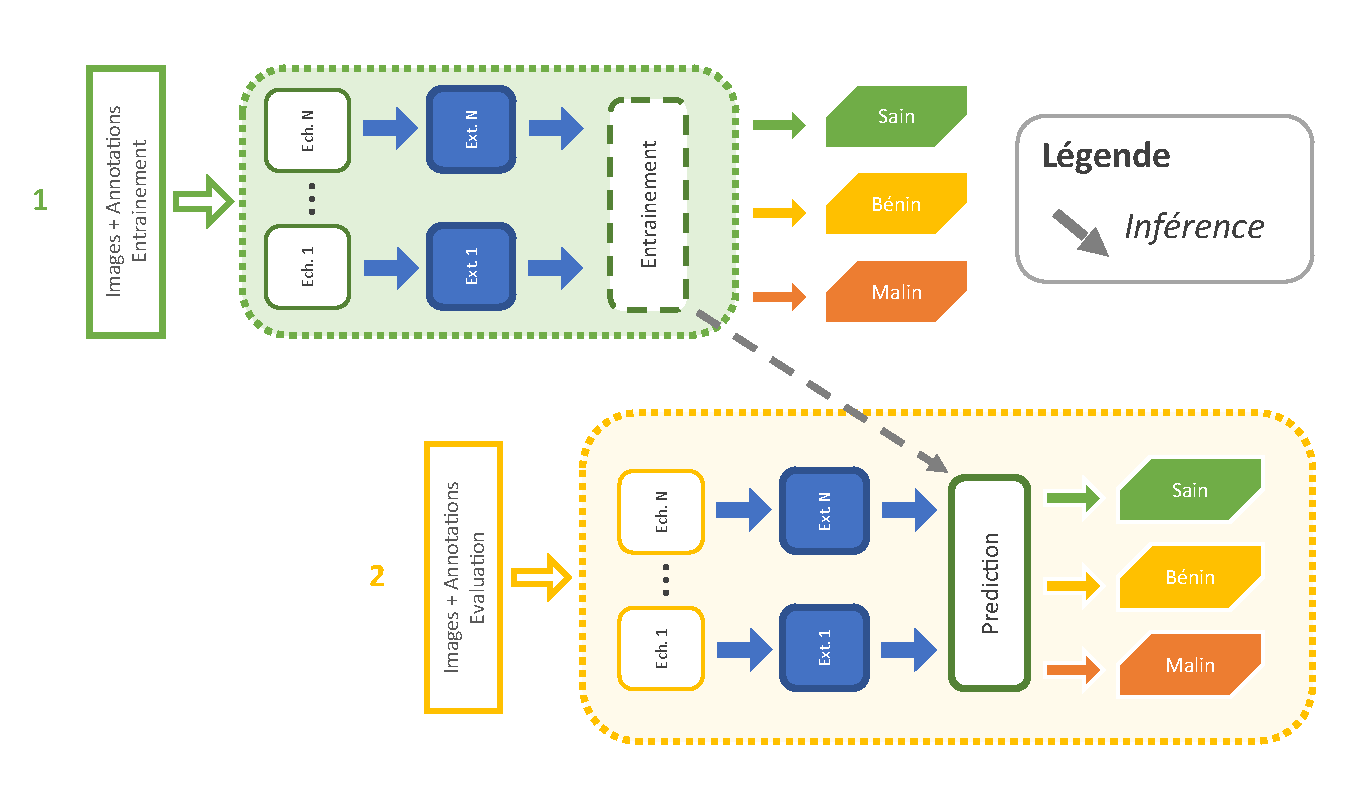
\includegraphics[width=\linewidth]{contents/chapter_5/resources/scheme_multiscale_features.pdf}
    \caption{Schéma de représentation du système multi-échelles sur base d'extraction puis de agrégation des caractéristiques avant classification.}
    \label{fig:scheme_multiscale_features}
\end{figure}\par

\begin{figure}[H]
    \centering
    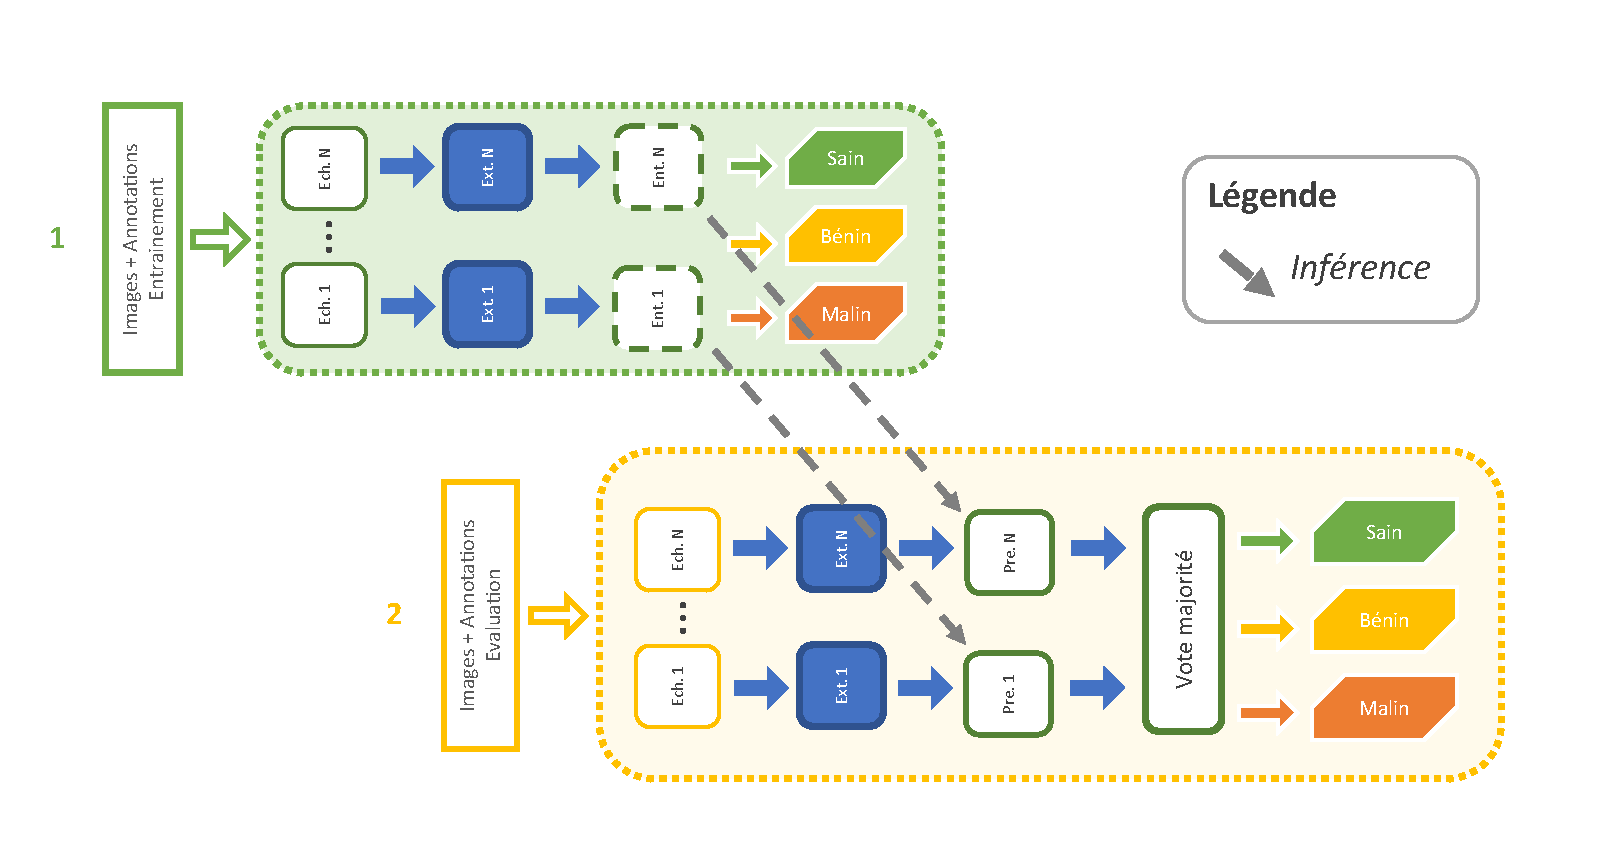
\includegraphics[width=\linewidth]{contents/chapter_5/resources/scheme_multiscale_decision.pdf}
    \caption{Schéma de représentation du système multi-échelles, sur base d'extractions et de classification à chaque échelle respective et par agrégation des décisions.}
    \label{fig:scheme_multiscale_decision}
\end{figure}\par

\subsection{Approche par fenêtre glissante}
Ces types d'approches ont été récemment utilisées à but de détection spatiale d'objet par l'utilisation de méthode d'apprentissage profond. A des fins médicales, ces approches ont permis la détection sur des images \gls{mri} du ventricule gauche~\cite{Helwan2017}.\par

Ces approches peuvent être également utilisées dans un contexte de classification lorsque la donnée comporte de l'information non directement liée aux annotations finales comme pour de la détection de cancer sur images histologiques par exemple~\cite{Hou2016,Alqudah2019}.\par

Les données images en notre possession corroborent avec ce type de schéma, puisque celle-ci sont soumise à un label global pour lesquels une hiérarchie à été mise en place. Pour rappel, un label malin qualifiera une donnée comportant au minimum des tissus typique d'une pathologie maligne mais pourra également comporter des tissus bénin et sain, et une annotation bénigne ne comportera que des tissus bénin ou sain.\par

Nous opterons pour un schéma de type supervisé de type approche de détection à faible échelle suivi d'une agrégation des décisions tel qu'employé dans certains travaux~\cite{Alqudah2019}. En effet, les données en notre possession nous permettent l'accès à des annotations de tissus de plus bas niveau réalisées par un spécialiste selon les même trois critères d'annotation.\par

Afin de mettre en oeuvre le schéma de détection à basse échelle, nous appliquerons les techniques jugées les plus pertinentes du chapitre précédent. Nous emploierons pour cela un schéma de classification comme sur la \Cref{fig:scheme_multiscale_decision}. De plus, n'ayant pas de critères de tailles optimum, nous feront varier ces paramètres afin d'étudier leur impact sur la classification. ces paramètres sont visible sur la \Cref{tab:sliding_window_parameters}.\par

\begin{figure}[H]
    \centering
    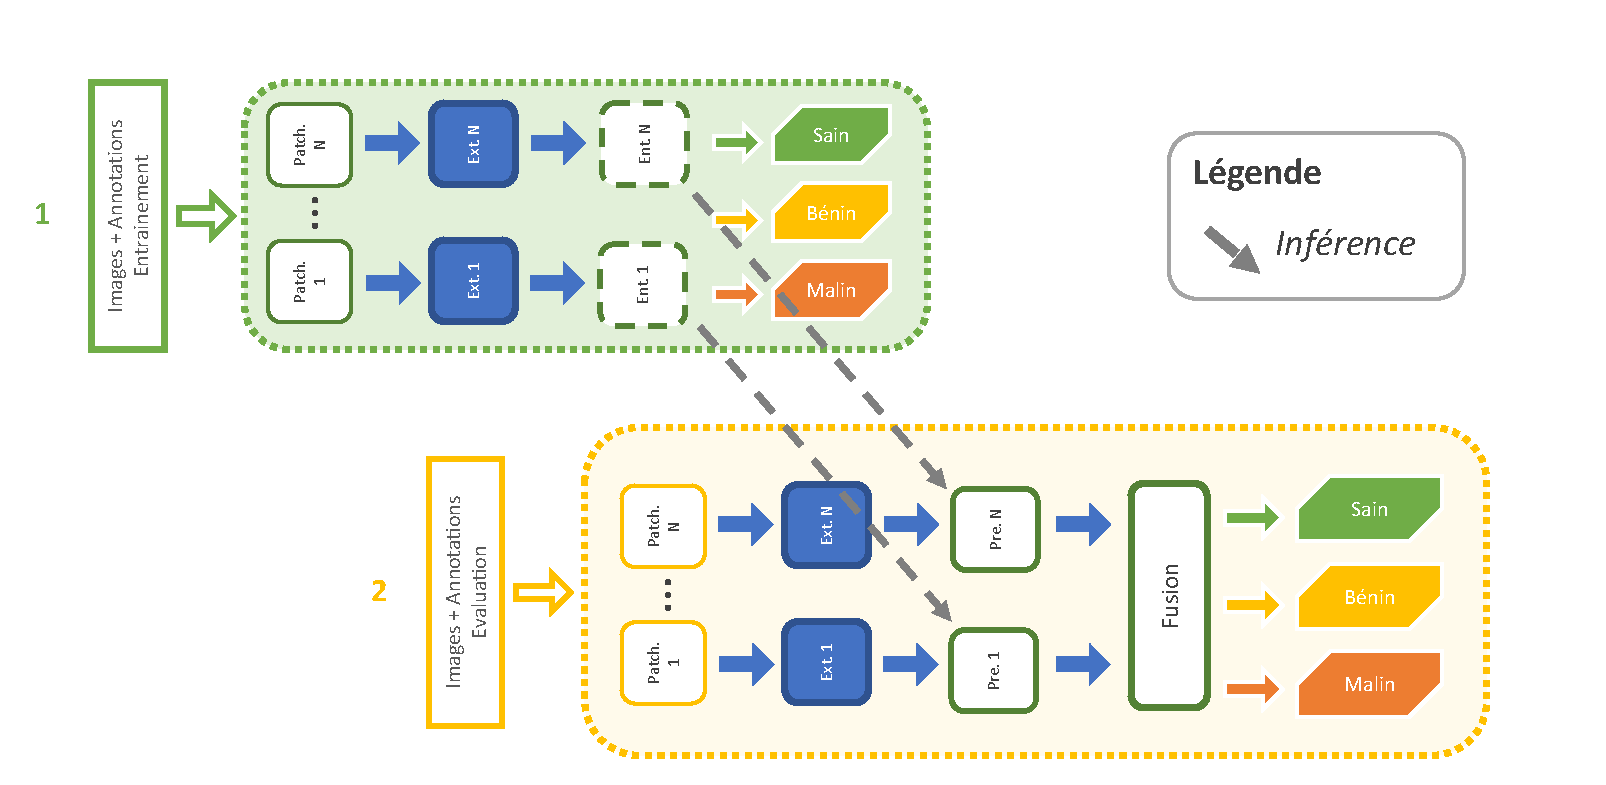
\includegraphics[width=\linewidth]{contents/chapter_5/resources/scheme_sliding_features.pdf}
    \caption{Schéma de représentation du système multi-échelles, sur base d'extractions et de classification à chaque échelle respective et par agrégation des décisions.}
    \label{fig:scheme_multiscale_decision}
\end{figure}\par

\begin{table}[H]
    \centering
    \begin{tabular*}{0.6\linewidth}{l@{\extracolsep{\fill}}l}
    \toprule
    \textbf{Résolution spatiale}& \textbf{Chevauchement}   \\ \hline
    250*250                     & 0\%                      \\ \hline
    250*250                     & 25\%                     \\ \hline
    250*250                     & 50\%                     \\ \hline 
    500*500                     & 0\%                      \\ \hline
    500*500                     & 25\%                     \\ \hline
    500*500                     & 50\%                     \\
    \bottomrule
    \end{tabular*}
    \caption{Paramètres appliqués à l'approche par fenêtre glissante.}
    \label{tab:sliding_window_parameters}
\end{table}\par

\section{Réglage fin de réseaux de convolution}
Dans cette partie, nous considérerons l'utilisation du réglage fin des \gls{cnn} adapté à notre problématique de classification d'images \gls{rcm}. Pour cela, nous nous consacrerons à ses divers aspects à l'aide de sous parties respectives propre à chaque concept. Nous débuterons par une présentation du réglage fin et des architectures que nous considérerons. Puis nous aborderons diverses techniques que nous mettrons en oeuvre, dont :
\begin{inlinerate}
    \item l'augmentation de données,
    \item le programme d'apprentissage,
    \item et la fonction de coût.
\end{inlinerate}\par

\subsection{Présentation générale}
Le réglage fin est une extension de l'apprentissage par transfert dans lequel est ajouté une ou des couches de classification adaptées au problème traité, et dans lequel tout ou partie du réseau est ré-entraîné à partir des poids existants. Ce mode d'apprentissage est utilisé lorsque les données propre au nouveau problème sont suffisantes, et permet d'obtenir un réseau plus adapté au nouveau problème.\par

Concernant les architectures que nous évaluerons dans ce chapitre, le travail mené par Park~\cite{Park2019} privélgie l'utilisation d'une architecture ResNet 50~\cite{He2016}. Néanmoins, lors du \Cref{chap:chapter_4} nous avons pu déterminer que l'architecture Inception-ResNet~\cite{Szegedy2017} utilisant un couche de Global Average Pooling et pré-entraîné sur la base ImageNet, semblait la plus judicieuse pour la classification de nos données.\par

A ce propos, aucune information n'est stipulée sur le type de Pooling employé par ce travail~\cite{Park2019}. Nous pouvons supposer l'utilisation d'une couche de Global Pooling basé sur la moyenne, couramment utilisée notamment pour de la visualisation de \gls{cnn} comme le propose ce travail.\par

\subsection{Augmentation de données}
Nous parlerons dans cette partie d'augmentation de données au sens de traitements appliqués au données d'entrées et non de création d'échantillons virtuels à partir de l'espace des caractéristiques pour corriger les problèmes de balancements~\cite{Wong2016}. Ainsi, nous considérerons l'augmentation de données comme une technique permettant de contrer le sur-apprentissage dans ce travail.\par


Ainsi, cette transformation est appliquée aux données d'entraînement afin d'apporter des variations.\par

~\cite{taylor2018}
\subsection{Programme d'apprentissage}
Le programme d'apprentissage ou \textit{Curriculum Learning} est une démarche visant par analogie à l'humain, à entraîner tout \gls{dnn} en proposant diverses tâches intermédiaires avec une difficulté croissante, afin d'accomplir avec une plus grande efficacité une tâche plus complexe. La raison technique recherché par cette méthode, est de proposer un espace de recherche plus simples des afin de trouver un meilleur minimum local comme l'ont suggéré ses premiers auteurs~\cite{Bengio2009}.\par

De récents travaux sur des images médicales, issue de rayons X (images en niveau de gris) ont permis par cette approche d'augmenter les performance de détection de \gls{cnn} sur des cancer du sein~\cite{Lotter2017} ou encore des cancers et autres pathologies pulmonaires~\cite{Park2019}. Le principe suivi par ces deux travaux, est de procéder à l'extraction de sous images de taille restreinte autour des dites lésions avérées, mais gardant la même propriété d'échelle. En effet, la gestion d'une même donnée à échelles multiples sur \gls{cnn} est un problème largement traité de la littérature non aisé~\cite{Noord2017}.\par

Ainsi nous emploierons à cet effet notre base d'images originale couplé aux sous images associées pour gérer cette tâche.\par

\subsection{Fonction de coût}
La fonction de coût est autre aspect que nous avons tenté de mener à bien dans ce travail.
~\cite{Park2019}
~\cite{Barbu2018}

\subsection{Carte d'activation de classe}
~\cite{jia2017}
\section{Analyse des résultats}